\documentclass[12pt]{report}
\usepackage[utf8]{inputenc}
\usepackage[russian]{babel}
%\usepackage[14pt]{extsizes}
\usepackage{listings}
\usepackage{graphicx}
\usepackage{amsmath,amsfonts,amssymb,amsthm,mathtools} 
\usepackage{pgfplots}
\usepackage{filecontents}
\usepackage{float}
\usepackage{indentfirst}
\usepackage{eucal}
\usepackage{enumitem}
%s\documentclass[openany]{book}
\frenchspacing

\usepackage{indentfirst} % Красная строка

\usetikzlibrary{datavisualization}
\usetikzlibrary{datavisualization.formats.functions}

\usepackage{amsmath}


% Для листинга кода:
\lstset{ %
	language=c,                 % выбор языка для подсветки (здесь это С)
	basicstyle=\small\sffamily, % размер и начертание шрифта для подсветки кода
	numbers=left,               % где поставить нумерацию строк (слева\справа)
	numberstyle=\tiny,           % размер шрифта для номеров строк
	stepnumber=1,                   % размер шага между двумя номерами строк
	numbersep=5pt,                % как далеко отстоят номера строк от подсвечиваемого кода
	showspaces=false,            % показывать или нет пробелы специальными отступами
	showstringspaces=false,      % показывать или нет пробелы в строках
	showtabs=false,             % показывать или нет табуляцию в строках
	frame=single,              % рисовать рамку вокруг кода
	tabsize=2,                 % размер табуляции по умолчанию равен 2 пробелам
	captionpos=t,              % позиция заголовка вверху [t] или внизу [b] 
	breaklines=true,           % автоматически переносить строки (да\нет)
	breakatwhitespace=false, % переносить строки только если есть пробел
	escapeinside={\#*}{*)}   % если нужно добавить комментарии в коде
}


\usepackage[left=2cm,right=2cm, top=2cm,bottom=2cm,bindingoffset=0cm]{geometry}
% Для измененных титулов глав:
\usepackage{titlesec, blindtext, color} % подключаем нужные пакеты
\definecolor{gray75}{gray}{0.25} % определяем цвет
\newcommand{\hsp}{\hspace{20pt}} % длина линии в 20pt
% titleformat определяет стиль
\titleformat{\chapter}[hang]{\Huge\bfseries}{\thechapter\hsp\textcolor{gray75}{|}\hsp}{0pt}{\Huge\bfseries}


% plot
\usepackage{pgfplots}
\usepackage{filecontents}
\usetikzlibrary{datavisualization}
\usetikzlibrary{datavisualization.formats.functions}

\begin{document}

\thispagestyle{empty}
\begin{titlepage}

\noindent \begin{minipage}{0.15\textwidth}
	
\includegraphics[width=\linewidth]{img/b_logo}
	\end{minipage}
	\noindent\begin{minipage}{0.9\textwidth}\centering
		\textbf{Министерство науки и высшего образования Российской Федерации}\\
		\textbf{Федеральное государственное бюджетное образовательное учреждение высшего образования}\\
		\textbf{~~~«Московский государственный технический университет имени Н.Э.~Баумана}\\
		\textbf{(национальный исследовательский университет)»}\\
		\textbf{(МГТУ им. Н.Э.~Баумана)}
	\end{minipage}
	
	\noindent\rule{18cm}{3pt}
	\newline\newline
	\noindent ФАКУЛЬТЕТ $\underline{\text{~~~~~~~~~~~~~~~~~~~«Информатика и системы управления»~~~~~~~~~~~~~~}}$ \newline\newline
	\noindent КАФЕДРА $\underline{\text{«Программное обеспечение ЭВМ и информационные технологии»}}$\newline\newline\newline\newline\newline
	
	\begin{center}
		\noindent\begin{minipage}{1.1\textwidth}\centering
			\Large\textbf{  Отчет по лабораторной работе №2}\newline
			\textbf{по дисциплине <<Математическая статистика>>}\newline\newline
		\end{minipage}
	\end{center}
	
	\noindent\textbf{Тема} $\underline{\text{~~~~~~~~~~~~~~~~~~~~~~~~~~~~~~~Интервальные оценки~~~~~~~~~~~~~~~~~~~~~~~~~~~~~~~~~~~~~~~~~~~~~~~~~~~~~~~}}$\newline\newline
	\noindent\textbf{Группа} $\underline{\text{~~~~~~~~~~~~~~~~~~~~~~~~~~~~~~~~~~~~ИУ7-63Б~~~~~~~~~~~~~~~~~~~~~~~~~~~~~~~~~~~~~~~~~~~~~~~~~~~~~~~~~~~~~~~~~}}$\newline\newline
	\noindent\textbf{Студент} $\underline{\text{~~~~~~~~~~~~~~~~~~~~~~~~~~~~~~~~Сукочева А.~~~~~~~~~~~~~~~~~~~~~~~~~~~~~~~~~~~~~~~~~~~~~~~~~~~~~~~~~~~~~~}}$\newline\newline
	\noindent\textbf{Преподаватель} $\underline{\text{~~~~~~~~~~~~~~~~~~~~~Саркисян П.С.~~~~~~~~~~~~~~~~~~~~~~~~~~~~~~~~~~~~~~~~~~~~~~~~~~~~~~~~~~~}}$\newline\newline\newline
	
\begin{center}
	\vfill
	Москва~---~\the\year
	~г.
\end{center}

\end{titlepage}

\chapter{Задание}

\section{Цель работы}

\textbf{Цель работы:} построение доверительных интервалов для математического ожидания и дисперсии нормальной случайной величины.

\section{Содержание работы}

\begin{enumerate}
    \item Для выборки объема $n$ из нормальной генеральной совокупности $X$ реализовать в виде программы на ЭВМ
        \begin{enumerate}
            \item вычисление точечных оценок $\hat\mu(\vec X_n)$ и $S^2(\vec X_n)$ математического ожидания $MX$ и дисперсии $DX$ соответственно;
            \item вычисление нижней и верхней границ $\underline\mu(\vec X_n)$, $\overline\mu(\vec X_n)$ для $\gamma$-доверительного интервала для математического ожидания $MX$;
            \item вычисление нижней и верхней границ $\underline\sigma^2(\vec X_n)$, $\overline\sigma^2(\vec X_n)$ для $\gamma$-доверительного интервала для дисперсии $DX$;
        \end{enumerate}
    \item вычислить $\hat\mu$ и $S^2$ для выборки из индивидуального варианта;
    \item для заданного пользователем уровня доверия $\gamma$ и $N$ – объёма выборки из индивидуального варианта:
        \begin{enumerate}
            \item на координатной плоскости $Oyn$ построить прямую $y = \hat\mu(\vec{x_N})$, также графики функций $y = \hat\mu(\vec x_n)$, $y = \underline\mu(\vec x_n)$ и $y = \overline\mu(\vec x_n)$ как функций объема $n$ выборки, где $n$ изменяется от 1 до $N$;
            \item на другой координатной плоскости $Ozn$ построить прямую $z = S^2(\vec{x_N})$, также графики функций $z = S^2(\vec x_n)$, $z = \underline\sigma^2(\vec x_n)$ и $z = \overline\sigma^2(\vec x_n)$ как функций объема $n$ выборки, где $n$ изменяется от 1 до $N$.
        \end{enumerate}
\end{enumerate}

\chapter{Теоретическая часть}

\section{Определение $\gamma$-доверительного интервала для значения параметра распределения случайной величины}

Пусть:
1) $X$ - случайная величина, закон распределения которой
известен с точностью до неизвестного параметра $\theta$.

Закон распределения с.в. $X$ известен с точностью до $\theta$
означает, что известен общий вид закона распределения с.в. $X$, но этот закон
зависит от неизвестного параметра $\theta$.
Если задать некоторое значение $\theta$, 
то закон распределения с.в. X будет известен полностью

Интервальной оценкой с уровнем доверия $\gamma$ 
($\gamma$-доверительной интервальной оценкой) 
параметра $\theta$ называют пару статистик 
$\underline{\theta}(\vec X), \overline{\theta}(\vec X)$ таких, что

\begin{equation*}
    P\{\underline{\theta}(\vec X)<\theta<\overline{\theta}(\vec X)\}=\gamma
\end{equation*}

% Поскольку границы интервала являются случайными величинами, то для различных реализаций случайной выборки $\vec X$ статистики $\underline{\theta}(\vec X), \overline{\theta}(\vec X)$ могут принимать различные значения.

Доверительным интервалом с уровнем доверия $\gamma$ ($\gamma$-доверительным интервалом) называют интервал $(\underline{\theta}(\vec x), \overline{\theta}(\vec x))$, отвечающий выборочным значениям статистик $\underline{\theta}(\vec X), \overline{\theta}(\vec X)$.

\section{Формулы для вычисления границ \\ $\gamma$-доверительного интервала для математического ожидания и дисперсии нормальной случайной величины}

Статистику $\hat{\theta}(\vec{X})$ называют точечной оценкой параметра $\theta$,
если ее выборочное значение принимается в качестве параметра $\theta$.
Т.е. $\theta = \hat{\theta}(\vec{x})$ 

Формулы для вычисления границ $\gamma$-доверительного интервала для математического ожидания:

\begin{equation}
\underline\mu(\vec X_n)=\overline X + \frac{S(\vec X)t^{St(n-1)}_{\frac{1-\gamma}{2}}}{\sqrt{n}}
\end{equation}

\begin{equation}
\overline\mu(\vec X_n)=\overline X + \frac{S(\vec X)t^{St(n-1)}_{\frac{1+\gamma}{2}}}{\sqrt{n}}
\end{equation}

$\overline X$ -- точечная оценка математического ожидания;
$S(\vec X) = \sqrtsign{S^2(\vec X)}$ -- квадратный корень из точечной оценки дисперсии;
$n$ -- объем выборки;
$\gamma$ -- уровень доверия;
$t^{St(n-1)}_{\alpha}$ -- квантиль уровня $\alpha$ распределения Стьюдента с $n - 1$ степенями свободы.

Формулы для вычисления границ $\gamma$-доверительного интервала для дисперсии:

\begin{equation}
\underline\sigma(\vec X_n)= \frac{(n-1)S^2(\vec X)}{t^{\chi^2(n-1)}_{\frac{1+\gamma}{2}}}
\end{equation}

\begin{equation}
\overline\sigma(\vec X_n)= \frac{(n-1)S^2(\vec X)}{t^{\chi^2(n-1)}_{\frac{1-\gamma}{2}}}
\end{equation}

$S^2(\vec X)$ -- точечная оценка дисперсии;
$n$ -- объем выборки;
$\gamma$ -- уровень доверия;
$t^{\chi^2(n-1)}_{\alpha}$ -- квантиль уровня $\alpha$ распределения $\chi^2(n-1)$ с $n - 1$ степенями свободы.


\chapter{Практическая часть}

\begin{figure}[ht!]	\centering{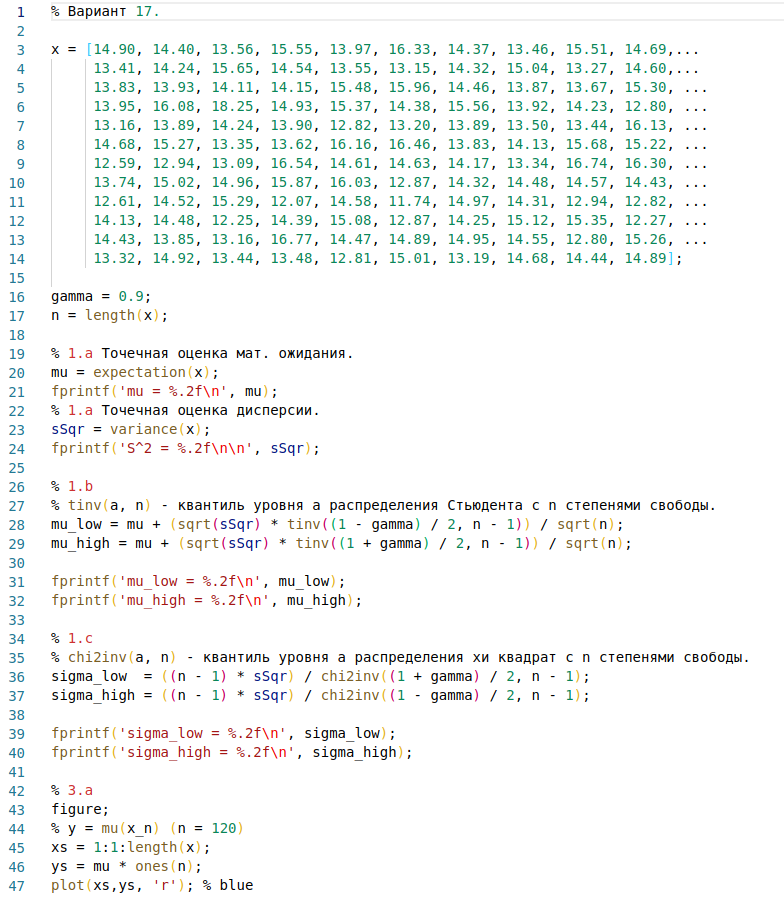
\includegraphics[width=0.8\textwidth]{img/code_1.png}}\end{figure}
\begin{figure}[ht!]	\centering{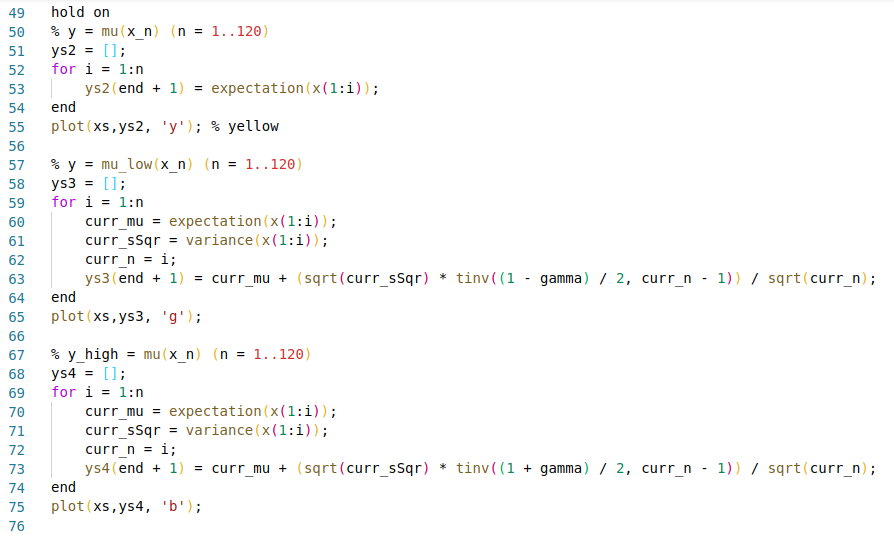
\includegraphics[width=0.8\textwidth]{img/code_2.png}}\end{figure}
\begin{figure}[ht!]	\centering{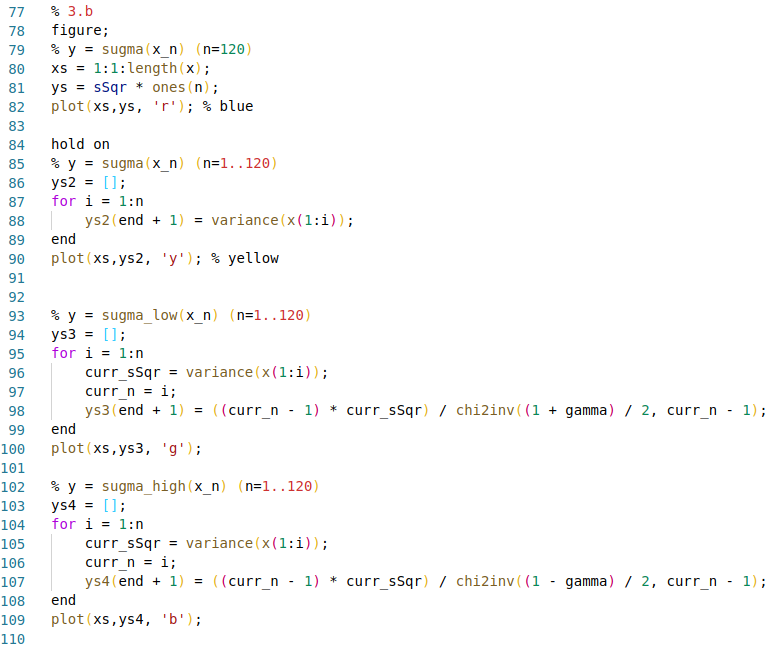
\includegraphics[width=0.8\textwidth]{img/code_3.png}}\end{figure}
\begin{figure}[ht!]	\centering{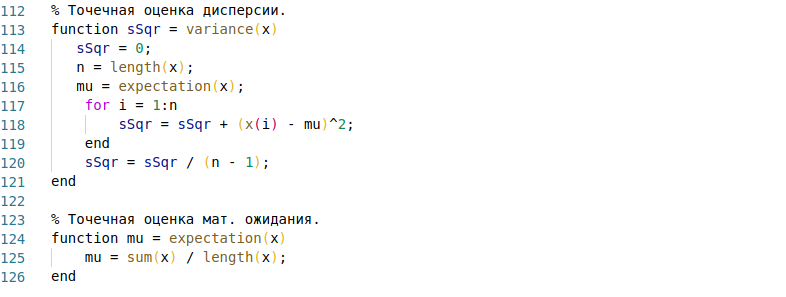
\includegraphics[width=0.8\textwidth]{img/code_4.png}}\end{figure}

\chapter{Экспериментальная часть}

\section{Результаты расчетов}

\begin{equation*}
    \hat\mu(\vec x_n) = 14,35\\
\end{equation*}
\begin{equation*}
    S^2(\vec x_n) = 1,28\\
\end{equation*}
\begin{equation*}
    \underline\mu(\vec x_n) = -14,18\\
\end{equation*}
\begin{equation*}
    \overline\mu(\vec x_n) = 14,52\\
\end{equation*}
\begin{equation*}
    \underline{S^2}(\vec x_n) = 1.05\\
\end{equation*}
\begin{equation*}
    \overline{S^2}(\vec x_n) = 1.6\\
\end{equation*}

\begin{figure}[ht!]	
	\centering{
		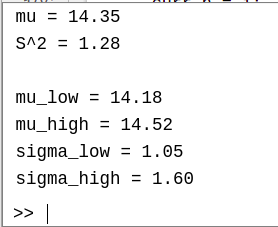
\includegraphics[width=0.3\textwidth]{img/res_1.png}
		\caption{Результаты расчетов}}
\end{figure}

\newpage

\begin{figure}[ht!]	
	\centering{
		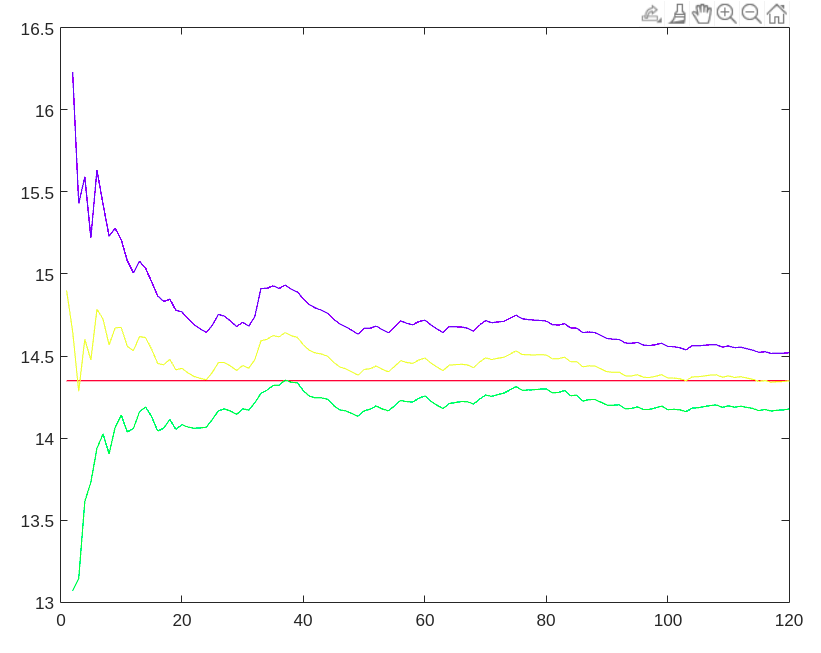
\includegraphics[width=0.7\textwidth]{img/res_2.png}
		\caption{Прямая $y(n) = \hat\mu(\vec x_N)$, а также графики функций  $y(n) = \hat\mu(\vec x_n)$, $y(n) = \underline\mu(\vec x_n)$, $y(n) = \overline\mu(\vec x_n)$ как функций объема $n$ выборки, где $n$ изменяется от 1 до $N$}}
\end{figure}


\begin{figure}[ht!]	
	\centering{
		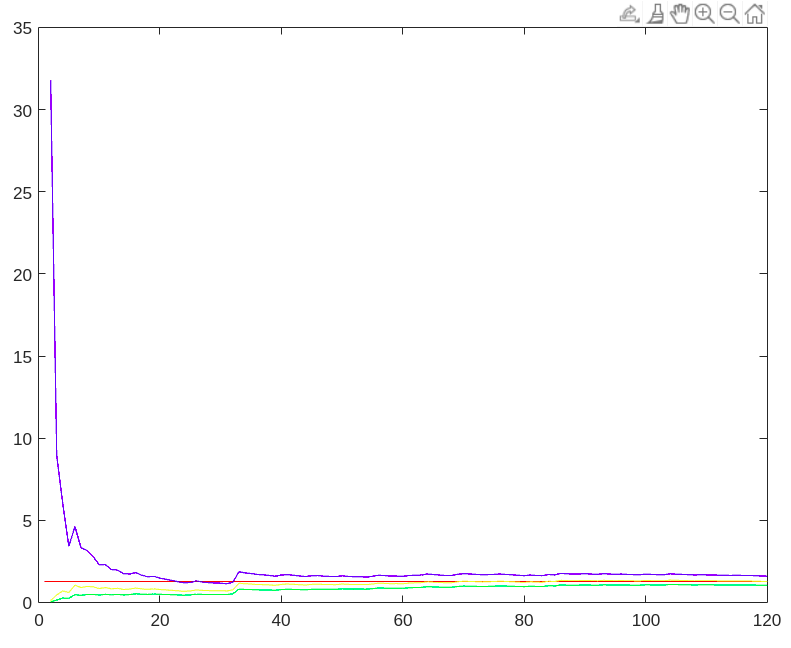
\includegraphics[width=0.7\textwidth]{img/res_3.png}
		\caption{Прямая $z(n) = \hat S^2(\vec x_N)$, а также графики функций $z(n) = \hat S^2(\vec x_n)$, $z(n) = \underline \sigma^2(\vec x_n)$, $z(n) = \overline \sigma^2(\vec x_n)$ как функций объема $n$ выборки, где $n$ изменяется от 1 до $N$}}
\end{figure}


\end{document}
